
\documentclass[a4paper,12pt]{article}
%%%%%%%%%%%%%%%%%%%%%%%%%%%%%%%%%%%%%%%%%%%%%%%%%%%%%%%%%%%%%%%%%%%%%%%%%%%%%%%%%%%%%%%%%%%%%%%%%%%%%%%%%%%%%%%%%%%%%%%%%%%%%%%%%%%%%%%%%%%%%%%%%%%%%%%%%%%%%%%%%%%%%%%%%%%%%%%%%%%%%%%%%%%%%%%%%%%%%%%%%%%%%%%%%%%%%%%%%%%%%%%%%%%%%%%%%%%%%%%%%%%%%%%%%%%%
\usepackage{eurosym}
\usepackage{vmargin}
\usepackage{amsmath}
\usepackage{graphics}
\usepackage{epsfig}
\usepackage{framed}
\usepackage{subfigure}
\usepackage{fancyhdr}

\setcounter{MaxMatrixCols}{10}
%TCIDATA{OutputFilter=LATEX.DLL}
%TCIDATA{Version=5.00.0.2570}
%TCIDATA{<META NAME="SaveForMode"CONTENT="1">}
%TCIDATA{LastRevised=Wednesday, February 23, 201113:24:34}
%TCIDATA{<META NAME="GraphicsSave" CONTENT="32">}
%TCIDATA{Language=American English}

\pagestyle{fancy}
\setmarginsrb{20mm}{0mm}{20mm}{25mm}{12mm}{11mm}{0mm}{11mm}
\lhead{MA4128} \rhead{Kevin O'Brien} \chead{Binary Classification} %\input{tcilatex}

%http://www.electronics.dit.ie/staff/ysemenova/Opto2/CO_IntroLab.pdf
\begin{document}
	\section*{Binary Classification}
Classification is the problem of identifying to which of a set of categories
(sub-populations) a new observation belongs, on the basis of a training set
of data containing observations (or instances) whose category membership is
known. 

Binary Classification is the task of classifying the members of a given set of objects into two groups on the basis
if them having a particular set of characteristics.



% Logisticn Rege Discriminant analysis is an example of a classification method.
\begin{itemize}
	\item  To train (create) a classifier, the fitting function estimates the parameters
	of a Gaussian distribution for each class.
	\item  To predict the classes of new data, the trained classifier finds the class
	with the smallest misclassification cost.
\end{itemize}


	
	

	\subsection*{Definitions}
	\textbf{Accuracy Rate}\\
	The accuracy rate calculates the proportion ofobservations being allocated to the \textbf{correct} group by the predictive model. It is calculated as follows:
	\[ \frac{
		\mbox{Number of Correct Classifications }}{\mbox{Total Number of Classifications }}  = \frac{TP + TN}{TP+FP+TN+FN}\]
	
	
	\noindent \textbf{Misclassification Rate}\\
	The misclassification rate calculates the proportion ofobservations being allocated to the \textbf{incorrect} group by the predictive model. It is calculated as follows:
	\[ \frac{
		\mbox{Number of Incorrect Classifications }}{\mbox{Total Number of Classifications }}  = \frac{FP + FN}{TP+FP+TN+FN}\]

%%%%%%%%%%%%%%%%%%%%%%%%%%%%%%%%%%%%%%%%%%%%%%%%%%%%%%%%%%%%%%%%%%%%%%%%%%%%%%%%%%%%%%%%%%

\subsection*{Sensitivity and Specificity}
\begin{itemize}
	\item Sensitivity and specificity are statistical measures of the performance of a binary classification test, also known in statistics as classification function. Sensitivity (also called the true positive rate, or the recall rate in some fields) measures the proportion of actual positives which are correctly identified as such (e.g., the percentage of sick people who are correctly identified as having the condition), and is complementary to the false negative rate.
	\item  Specificity (sometimes called the true negative rate) measures the proportion of negatives which are correctly identified as such (e.g., the percentage of healthy people who are correctly identified as not having the condition), and is complementary to the false positive rate.
	\item A perfect predictor would be described as 100\% sensitive (e.g., all sick are identified as sick) and 100\% specific (e.g., all healthy are identified as healthy); however, theoretically any predictor will possess a minimum error bound known as the \textbf{\textit{Bayes error rate}}.
	\item For any test, there is usually a trade-off between the measures. For instance, in an airport security setting in which one is testing for potential threats to safety, scanners may be set to trigger on low-risk items like belt buckles and keys (low specificity), in order to reduce the risk of missing objects that do pose a threat to the aircraft and those aboard (high sensitivity). 
	\item This trade-off can be represented graphically as a \textbf{\textit{receiver operating characteristic curve}}.
	
\end{itemize}

\subsection*{Sensitivity and Specificity}
Sensitivity and specificity are measures of the performance of a binary classification
test.
\begin{itemize}
	\item \textbf{Sensitivity} (also called the true positive rate, or the \textbf{recall} rate) measures
	the proportion of actual positives which are correctly identified
	as such (e.g. the percentage of sick people who are correctly identified
	as having the condition).
	
	\[ \mbox{Sensitivity (Recall)} = \frac{TP}{TP +FN}\]
	
	\begin{itemize}
		\item \textit{(Remark: We will use the terms Sensitivity and Recall interchangeably.
			Sensitivity is more commonly used in a medical context, while recall is more
			commonly used in data science.)}
	\end{itemize}
	\item \textbf{Specificity} measures the proportion of negatives which are correctly
	identified as such (e.g. the percentage of healthy people who are correctly
	identified as not having the condition, sometimes called the true
	negative rate).
	
	\[ \mbox{Specificity} = \frac{TN}{TP +FN}\]
	
	\begin{itemize}
		\item \textit{(Remark: Not commonly used in Data Sciences, and NOT a synoym for Precision)}
	\end{itemize}
\end{itemize}
\newpage




\subsection*{Types I and II Error}
A type I error is the incorrect rejection of a true null hypothesis. A type
II error is the failure to reject a false null hypothesis. A type I error is a
false positive. Usually a type I error leads one to conclude that a thing or
relationship exists when really it doesn’t. A type II error is a false negative.
\begin{figure}[h!]
	\centering
	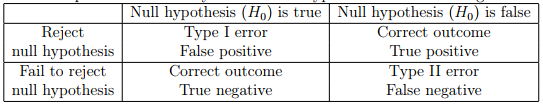
\includegraphics[width=0.7\linewidth]{Table}
	% \caption{}
	% \label{fig:table}
\end{figure}

\subsection*{False Positive and False Negative Error}

\begin{itemize}
	\item 
	A false positive error, commonly called a ``\textbf{false alarm}``, is a result that indicates
	a given condition has been fulfilled, when it actually has not been
	fulfilled. A false positive error is a Type I error % where the test is checking a single condition, and results in an affirmative or negative decision usually
	% designated as ”true or false”.
	\item  A false negative error is where a test result indicates that a condition
	failed, while it actually was successful. A false negative error is a Type II
	error.% occurring in test steps where a single condition is checked for and the 	result can either be positive or negative.
\end{itemize}




\subsection*{Accuracy, Recall and Precision: An Example}
Calculating precision and recall is actually quite easy. Imagine there are
135 positive cases among 10,000 cases. You want to predict which ones are
positive, and you pick 265 to have a better chance of catching many of the
135 positive cases. You record the IDs of your predictions, and when you
get the actual results you sum up how many times you were right or wrong.
There are four ways of being right or wrong:
\begin{itemize}
\item TN / True Negative: case was negative and predicted negative
\item TP / True Positive: case was positive and predicted positive
\item  FN / False Negative: case was positive but predicted negative
\item FP / False Positive: case was negative but predicted positive
\end{itemize}
Now count how many of the 10,000 cases fall in each category:
\begin{center}
\begin{tabular}{|c|c|c|}
  & Predicted Negative & Predicted Positive \\ \hline
Negative Cases & TN: 9,700 & FP: 165 \\ \hline
Positive Cases &  FN: 35 & TP: 100 \\ \hline
\end{tabular}
\end{center}
What percent of your predictions were correct?
\begin{itemize}
	\item The accuracy was (9,760+60) out of 10,000 = 98.00\%\\
	What percent of the positive cases did you catch?
	\item The recall was 100 out of 135 = 74.07\%
	What percent of positive predictions were correct?\\
	\item The precision was 100 out of 265 = 37.74\%
	What percent of negative predictions were correct? \\
	\item The specifity was 9700 out of 9735 = 99.64\%
\end{itemize}

\subsection*{The F Score}
The F-score or F-measure is a measure of a classification procedure’s accuracy.
It considers both the precision and the recall to compute the score.
\[ F = \frac{2 \times \mbox{precision} \times \mbox{recall}}{\mbox{precision} + \mbox{recall}}\]


\section*{ Cross Validation}
When prediction
is perfect all cases will lie on the diagonal. The percentage of cases on the
diagonal is the percentage of correct classifications. The cross validated set of
data is a more honest presentation of the power of the discriminant function
than that provided by the original classifications and often produces a poorer
outcome. The cross validation is often termed a jack-knife classification, in
that it successively classifies all cases but one to develop a discriminant
function and then categorizes the case that was left out. This process is
repeated with each case left out in turn.This is known as leave-1-out cross
validation.
This cross validation produces a more reliable function. The argument
behind it is that one should not use the case you are trying to predict as part
of the categorization process.
\subsection*{Error Rates}
\begin{itemize}
	\item We can evaluate error rates by means of a training sample (to construct the
	discrimination rule) and a test sample.
	\item An optimistic error rate is obtained by reclassifying the training data. (In
	the training data sets, how many cases were misclassified). This is known
	as the apparent error rate.
	\item The apparent error rate is obtained by using in the training set to estimate
	the error rates. It can be severely optimistically biased, particularly for
	complex classifiers, and in the presence of over-fitted models.
	\item If an independent test sample is used for classifying, we arrive at the true
	error rate.
	\item The true error rate (or conditional error rate) of a classifier is the
	expected probability of misclassifying a randomly selected pattern. It is the
	error rate of an infinitely large test set drawn from the same distribution as
	the training data.
\end{itemize}

\subsection*{Misclassification Cost}
As in all statistical procedures it is helpful to use diagnostic procedures to
asses the efficacy of the discriminant analysis. We use cross-validation to
assess the classification probability. Typically you are going to have some
prior rule as to what is an acceptable misclassification rate.
Those rules might involve things like, “what is the cost of misclassification?”
Consider a medical study where you might be able to diagnose cancer.
There are really two alternative costs. The cost of misclassifying someone
as having cancer when they don’t. This could cause a certain amount of emotional
grief. Additionally there would be the substantial cost of unnecessary
treatment.
\smallskip 
There is also the alternative cost of misclassifying someone as not having
cancer when in fact they do have it.
A good classification procedure should
\begin{itemize}
	\item result in few misclassifications
	\item take prior probabilities of occurrence into account
	\item consider the cost of misclassification
\end{itemize}
For example, suppose there tend to be more financially sound firms than
bankrupt firm. If we really believe that the prior probability of a financially
distressed and ultimately bankrupted firm is very small, then one should classify
a randomly selected firm as non-bankrupt unless the data overwhelmingly
favor bankruptcy.
\smallskip 
There are two costs associated with discriminant analysis classification:
The \textbf{true misclassification cost per class}, and the\textbf{ expected misclassification
	cost} (ECM) per observation.

\smallskip

Suppose there we have a binary classification system, with two classes:
class 1 and class 2. Suppose that classifying a class 1 object as belonging
to class 2 represents a more serious error than classifying a class 2 object as
belonging to class 1. There would an assignable cost to each error. c(i|j) is
the cost of classifying an observation into class j if its true class is i. The
costs of misclassification can be defined by a cost matrix.
\begin{center}
	
	\begin{tabular}{|c|c|c|}
		& Predicted & Predicted \\ 
		& Class 1 & Class 2 \\ \hline 
		Class 1 & 0&  c(2|1) \\ \hline 
		Class 2 & c(1|2) & 0 \\ \hline 
	\end{tabular}
\end{center}


\subsection*{ Expected Cost of Misclassification (ECM)}
Let p1 and p2 be the prior probability of class 1 and class 2 respectively.
Necessarily p1 + p2 = 1.

The conditional probability of classifying an object as class 1 when it is
in fact from class 2 is denoted p(1|2). Similarly the conditional probability
of classifying an object as class 2 when it is in fact from class 1 is denoted
$p(2|1)$.
\[ ECM = c(2|1)p(2|1)p1 + c(1|2)p(1|2)p2\]
(In other words: the sum of the cost of misclassification times the (joint)
probability of that misclassification.
A reasonable classification rule should have ECM as small as possible.
\subsection*{Misclassification Rate}
The misclassification rate calculates the proportion ofobservations being allocated to the \textbf{incorrect} group by the predictive model. It is calculated as follows:
\[ \frac{
	\mbox{Number of Incorrect Classifications }}{\mbox{Total Number of Classifications }} \]

\[ = \frac{FP + FN}{TP+FP+TN+FN}\]


%-----------------------------------------------------------------------------------%
\subsection*{Error Rates}
\begin{itemize}
\item We can evaluate error rates by means of a training sample (to construct the discrimination rule) and a test sample.

\item 
An optimistic error rate is obtained by reclassifying the training data. (In the \textbf{\textit{training data}} sets, how many cases were misclassified). This is known as the \textbf{apparent error rate}.

\item 
The apparent error rate is obtained by using in the training set to estimate
the error rates. It can be severely optimistically biased, particularly for complex classifiers, and in the presence of over-fitted models.

\item
If an independent test sample is used for classifying, we arrive at the  \textbf{true error rate}.The true error rate (or conditional error rate) of a classifier is the expected
probability of misclassifying a randomly selected pattern.
It is the error rate of an infinitely large test set drawn from the same distribution as the training data.

\end{itemize}
%%%%%%%%%%%%%%%%%%%%%%%%%%%%%%%%%%%%%%%%%%%%%%%
\end{document}
